\chapter{History of Routing}
\label{chap:hist}
\begin{flushright}
 \textit{\textquotedblleft Not all those who wander are lost.\textquotedblright}\\
\textit{-- J.R.R. Tolkien}
\end{flushright}
 %Tolkien's quote “Not all those who wander are lost.”
\ifpdf
      
\graphicspath{{2-HistoryOfRouting/Chapter1Figs/PNG/}{2-HistoryOfRouting/Chapter1Figs/PDF/}{2-HistoryOfRouting/Chapter1Figs/}}
\else
   
\graphicspath{{2-HistoryOfRouting/Chapter1Figs/EPS/}{2-HistoryOfRouting/Chapter1Figs/}}
\fi

\section{Networking Fundamentals}

% There are many different kinds of networks, and network technologies used to
% create them. The proliferation of networking methods has generally occurred for
% a very good reason: different needs require different solutions. The drawback of
% this is that there are so many different types of protocols and technologies for
% the networking student to understand! Before you can really compare these
% approaches, you need to understand some of the basic characteristics that make
% networks what they are. While network types may be quite dissimilar, they are
% often described and even contrasted on the basis of a number of common
% attributes.

%Computers and computing systems have come a long way over the past halfcentury. 

One of the most significant evolution of computer systems is the merging of computers with communication systems \cite{Tanenbaum}. The early model of a single mainframe computer serving just local users has been replaced with a globally distributed set of interconnected commodity machines. This new model is called a Computer Network. The interconnecting media, and the way they are exploited have also evolved.with time giving rise to countless network protocols.

%Computer centers where, once upon a time, users would bring their work to has been revolutionized. The mainframe has been replaced by large interconnection of commodity machines; this interconnection is called a Computer Network. 

Many communication solutions have emerged over the decades in response to different requirements and therefore there are innumerable network technologies used to support or create them. The main drawback of this situation is that there are also countless network protocols, and thereby it becomes virtually impossible to understand all of them. 

\subsection{Reference Models}

Networking software has been designed as layers, as shown in Figure \ref{fig:refmodel}, in an effort to reduce its complexity. The goal of each layer, in all networks, is to expose services to the higher layers via interfaces between each layer, thereby abstracting the implementation complexities. Such a design is extremely powerful, not only because each layer is free to define how it performs its objective but also it can be optimized or completely replaced without affecting other layers. Each layer on a host uses a protocol to communicate with the same layer on another host. A protocol is defined as an agreement by both communicating parties on how the information exchange should proceed.


\begin{figure}
  \centering
  \subfloat[The Reference Model.]{\label{fig:refmodel}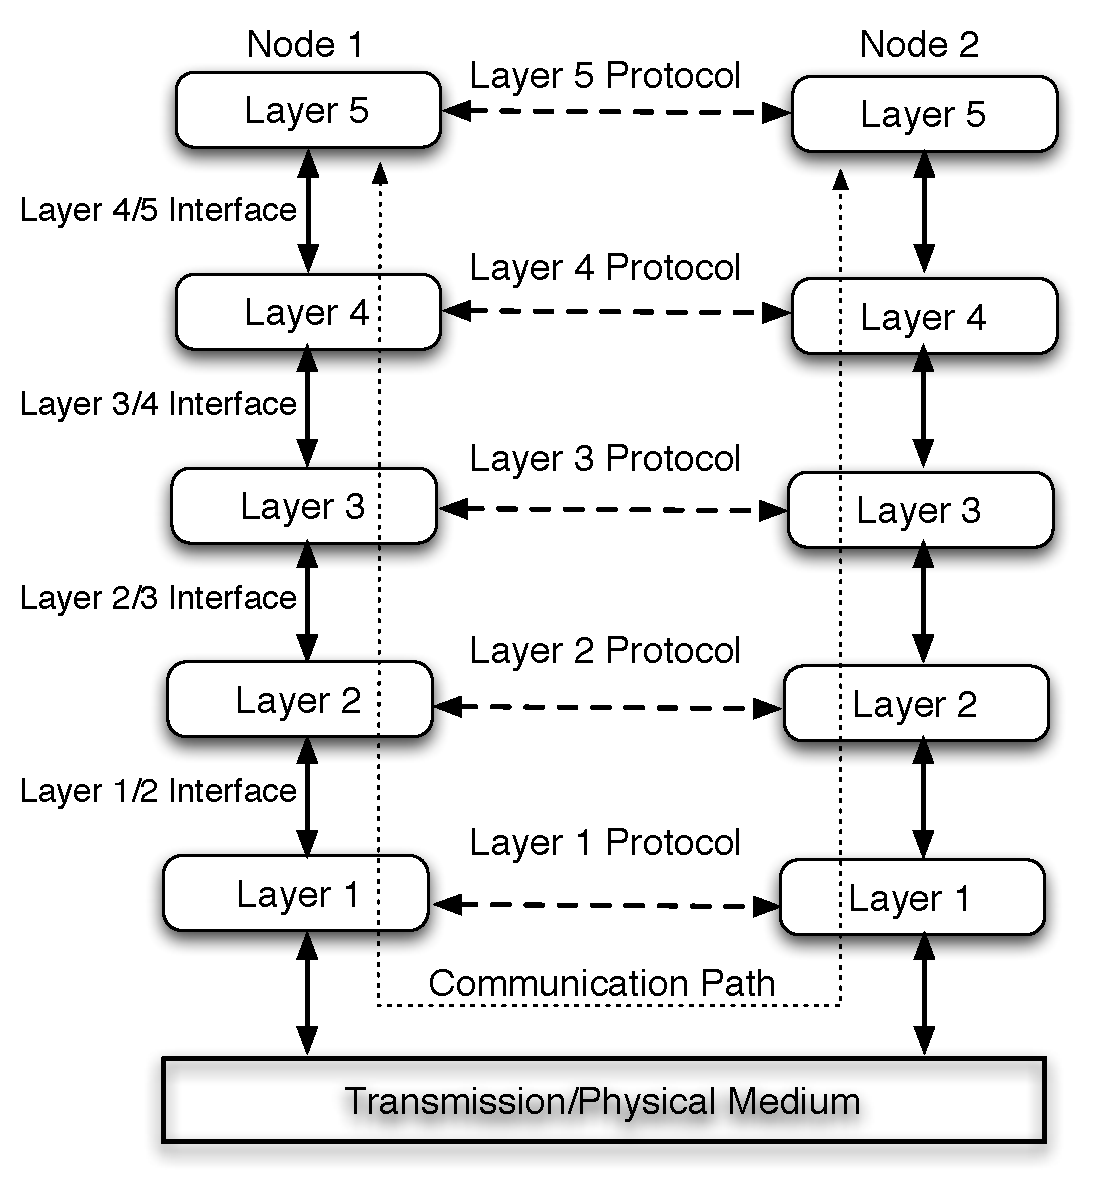
\includegraphics[scale=0.3]{RefModel}}                
  \subfloat[The OSI Model]{\label{fig:osimodel}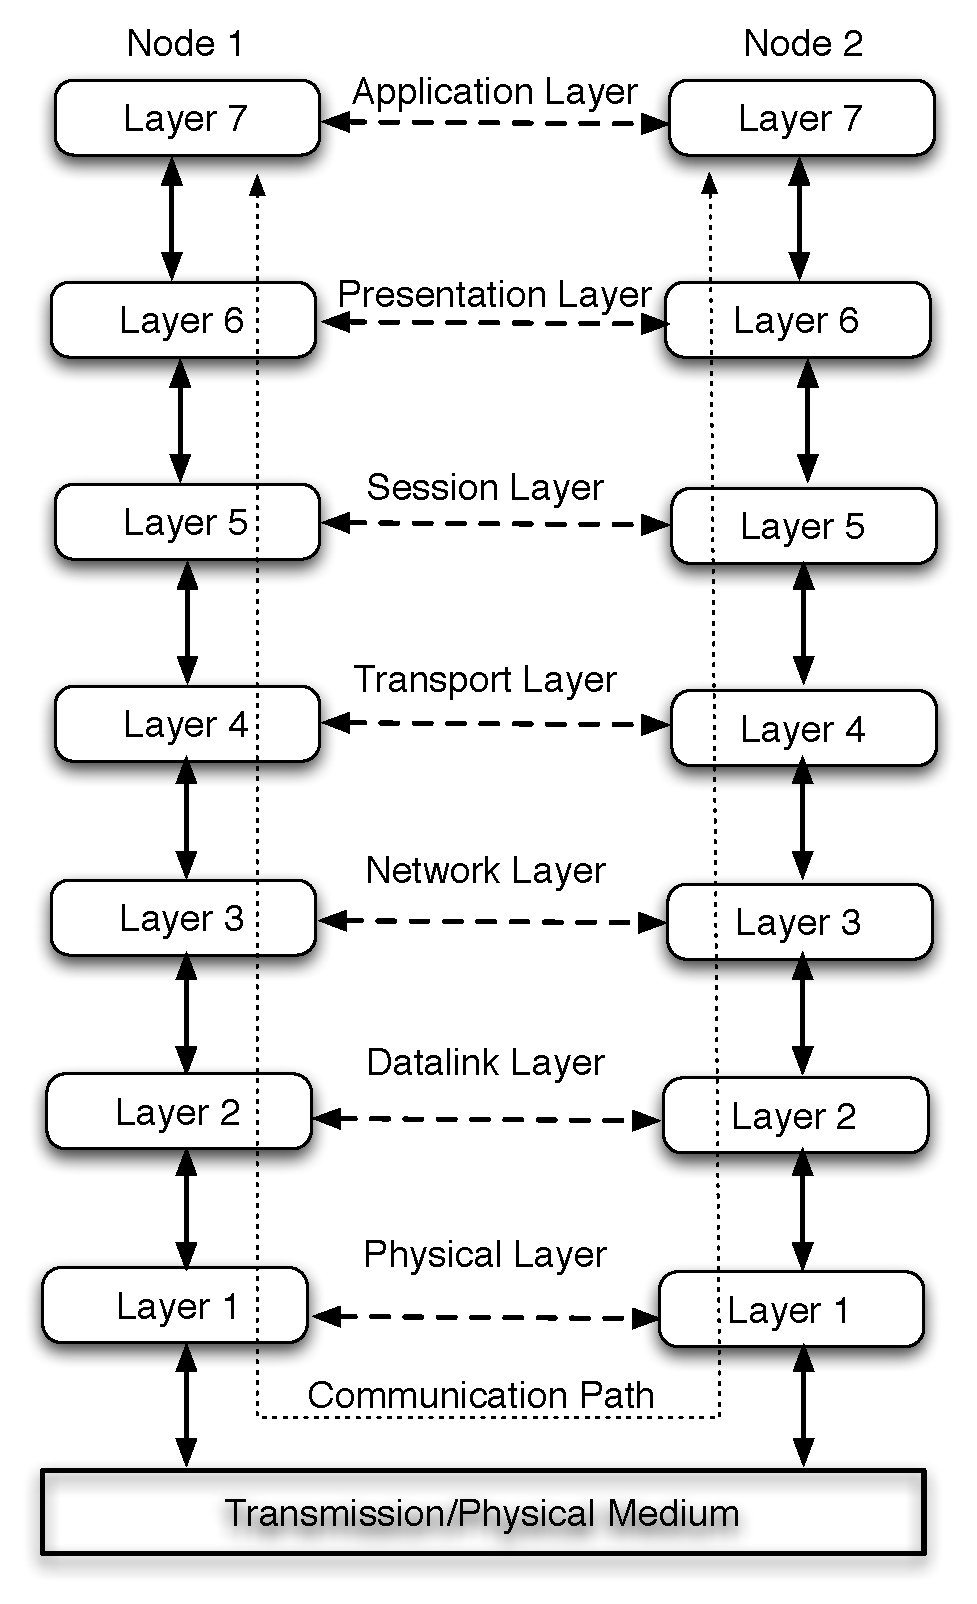
\includegraphics[scale=0.3]{OSIModel}}
  \caption{Inter-networking models}
  \label{fig:refmodels}
\end{figure}


%% Subfigure the refmodel and the osi model.
%ifigure{referencemodel}{0.45}{Reference Model (a) and OSI Model (b)}{fig:refmodel}

Figure \ref{fig:refmodels} depicts the layers, protocols and interfaces used to communicate between two nodes. Horizontal lines depict logical communication path, as no actual physical communication occurs horizontally, but rather physical communication occurs as shown by the dotted line, ie. via all the layers. 

In the next subsections, we will present two models; the OSI and the TCP/IP models. While the OSI model is general and the features addressed by each layer are still important, it is rarely used because of the bad timing of the standard ratification and its complexity. However, it is still the theoretical reference model for networks. On the other hand, the TCP/IP protocols are widely used, but the model is particular, and does not always provide a clear separation of interfaces and protocols.                                                       
                     

\subsubsection{The OSI Model}

The Open Systems Interconnection (OSI) reference model was originally developed by the International Standards Organization in an effort to standardize the protocols used in the model. Figure \ref{fig:osimodel}, shows the seven layers which make up the OSI stack. 

%\ifigure{OSI}{1}{The OSI Model.}{fig:osi}

Each layer in the OSI model performs a well defined function, and the boundaries are chosen to minimize the amount of information which has to be exchanged across the interfaces. 

We will now present the function of each layer:

\begin{enumerate}


 \item \textit{The Application Layer} is the layer which is closest to the user. Essentially this means that both this layer and the user interact with the software application.
 
 %HTTP (Hyper Text Transfer Protocol) for world wide web surfing, FTP (File Transfer protocol) for file transfer, SMTP (Simple Mail Transfer Protocol) for electronic mail, etc. Note that the protocols cited here 

 \item \textit{The Presentation Layer}, contrarily to the other lower level layers which are designed to shift bits around reliably, attempts to add syntax and semantics to to the information. It does this by providing function to operations that are performed often. 

 \item \textit{The Session Layer} enables users to establish sessions between themselves. For example, it would be used to login to a remote system or transfer a large document.
 
 \item \textit{The Transport Layer} has the basic role of obtaining data from the above session layer and splitting it up into smaller data units. These data units are then passed to the underlying network layer and the transport layer then makes sure the data arrives correctly at the other end.

 \item \textit{The Network Layer} handles and controls all the operations concerning a subnet. A particular issue is how a packet is routed from its source to its destination. These routes can either be determined statically or allocated dynamically. In this thesis we discuss different algorithms which are implemented in this layer.

 \item \textit{The Data Link Layer} has the task of obtaining the raw data from the physical layer and turning it into an input stream that seems error-free. This is accomplished by imposing that the sender split up the data into frames and transmit them sequentially. 


 \item \textit{The Physical Layer} is responsible for transmitting the raw bits over the physical medium. It is responsible for the actual translation of bits into electrical voltages or optical levels and vice versa.

\end{enumerate}


\subsubsection{The TCP/IP Model}

TCP/IP was designed for the ARPANET which was a project sponsored by the US Department of Defense (DoD). TCP/IP was built with a high degree of resiliency due to the fact that the DoD could have its installation attacked at any moment, and therefore wanted to keep communications alive as long as the end-hosts were still alive. The TCP/IP reference model, shown in Figure \ref{fig:tcpip}, was first defined by Cerf et al. \cite{CerfKahn}, and consists of four layers which we are going to detail below:

\ifigure{TCPModel}{0.7}{The TCP/IP Model}{fig:tcpip}

\begin{enumerate}

 \item \textit{The Application Layer} contains the same high level protocols described for the OSI application layer. The protocols used at this layer are denoted as Layer 7 protocols (analogy with the OSI layers), even if the TCP/IP stack only has four layers (five, depending how you consider the Host-to-Network 
Layer).

 \item \textit{The Transport Layer} provides the same functionality described by the OSI Transport layer, and its protocols are frequently denoted as Layer 4 protocols. Two end-to-end protocols are defined by the model: TCP (Transport Control Protocol) and UDP (User Datagram Protocol). While TCP is connection-oriented and provides a reliable (error free) end-to-end communication, UDP is a connectionless protocol which does not provide any guarantee on the integrity of the transmitted data. However, UDP is lightweight compared with TCP and also provides multicast capabilities (i.e. one-to-many transmission).


 \item \textit{The Internet Layer} defines the IP (Internet Protocol) protocol and packet format. This protocol is designed to deliver the IP packets over a network with multiple paths. As packets from the same conversation may follow different routes, experiencing different delays, there is no guarantee for preserving the order of IP packets. As the IP protocol provides functionality similar with that of the OSI network layer, it is often denoted as a Layer 3 protocol.


 \item \textit{The Host-to-Network Layer} is not precisely defined in the TCP/IP model except to state that the host must connect to the physical medium in order to send IP packets. The protocol, commonly, found here is the Medium Access Control Protocol, which provides addressing and medium access control mechanisms that make it possible for several hosts to communicate within a network.

\end{enumerate}


\subsection{Foundations of Ethernet.}

Ethernet is a technology which spans layers one and two of the OSI model, namely the physical layer and the datalink layer. Actually, the datalink layer has never changed since the introduction of Ethernet. The real beginning to Ethernet took place on the island of Hawaii in the early 1970s with a system named the ALOHA developed by the University of Hawaii \cite{aloha}. This system was constructed to allow radio communications between distant machines scattered over the island and a central IBM mainframe.

The ALOHA system allowed for a data rate of 9600 bits per second with fixed size frames transmitted sequentially. The mainframe would use a separate channel to convey acknowledgements of a successful transmission to sending hosts. If a terminal did not receive an acknowledgement after a fixed amount of time, it would timeout. Upon a timeout, the sending station would wait a random amount of time and attempt to retransmit. If two stations attempted to transmit simultaneously, the data arriving at the mainframe would appear corrupted due to the overlapping communications from the source stations. Such an event was referred to as a \textit{collision} causing both data packets to be lost and therefore neither station would receive an acknowledgement from the mainframe. The \textit{collision} and timeout mechanisms resulted in poor performance by the ALOHA protocol, only about 18\% of the bandwidth was ever usable \cite{Tanenbaum}.

In 1973, a researcher named Robert Metcalfe in Xerox's research laboratory in Palo Alto developed an improved version of the ALOHA system. This system, named Ethernet (Figure \ref{fig:ethernet}), was designed to interconnect computers in the laboratory. Ethernet was named after \textit{luminiferous ether}, which was thought to be the universal transmission medium for light at the end of the 19th century.

\ifigure{ethernet}{0.7}{The concept of Ethernet, as drawn originally by Bob Metcalfe.}{fig:ethernet}

With Ethernet came a new transmission medium, a thick yellow coaxial cable. Still the idea was the same as ALOHA, as the coaxial cable was the shared medium. Ethernet did not have a control channel as ALOHA did, so Metcalfe devised the Carrier Sense Multiple Access with Collision Detection (CSMA/CD) protocol \cite{Tanenbaum}, in order to better make use of the available bandwidth offered by this cable. 

\ifigure{CSMA}{0.6}{A simplified algorithm sketch for CSMA/CD}{fig:CSMA}

Figure \ref{fig:CSMA} shows a simplified flowchart of the CSMA/CD algorithm. Initially, a station must listen on the shared medium before taking a decision to transmit, as it can only transmit when the medium is free, otherwise it will cause a collision. Due to the propagation delay imposed by the shared medium, two stations may consider that the medium is free and start their transmission, thereby inadvertently causing a collision. The stations detect this collision and stop their transmissions immediately and wait a random amount of time before attempting a retransmission. The interval in which a collision may happen is referred  to as the collision window.

The maximal collision window is double the propagation time between the two ends of the network. In order for the collision mechanism to work correctly, the transmission time for the smallest frame has to be greater or equal to the collision window, if it is less then we obtain what is known as a collision fragment. It is therefore clear that a small collision window associated with the transmission of large frames would yield the maximum efficiency of the transmission medium. The Ethernet standard, however, defines the smallest and largest frame sizes possible. This in turn determines the theoretical efficiency of the network transmission, while real networks have more overhead as shown in \cite{EtherCapa}.

The Ethernet developed by Metcalfe and Xerox was so successful that Xerox, DEC and Intel drew up a standard for it which later became the base for IEEE 802.3 \cite{IEEE802.3, EtherGuide}. The transmission rate was set to 10 Mbps, the maximum and minimum frame sizes where set to 1518 and 64 bytes respectively. The official denomination 10BASE5 was adopted (10 Mbps data rate, base band transmission with network segments of 500 meters maximum). The shared medium was used for both directions thereby creating a half duplex network. In order to increase the maximum size of the network, devices called repeaters were introduced, which would clean and amplify the signal. 

\ifigure{EtherFrame}{0.6}{Structure of an 802.3 Ethernet Frame.}{fig:Ethernet}

The Ethernet IEEE standard \cite{IEEE802.3} defined the structure of the frame as shown in Figure \ref{fig:Ethernet}. The frame starts with a preamble, which is a special pattern allowing the receiver clock to synchronize with the incoming stream. The preamble is followed by the \textit{Start of Frame Delimiter (SFD)} which indicates the  immediate arrival of the frame. The source and destination fields are numbers which uniquely identify a device connected to the Ethernet network, although the destination field can contain special numbers that indicate that this communication is either multicast or broadcast. The length field is used to communicate the amount of data in the payload if it is less than 1500 otherwise this field is used to give information to higher layer on how to interpret the payload. If the payload carried is less than 46 bytes then it is padded with zeros in order to reach the minimum length of an Ethernet frame of 64 bytes. The \textit{Cyclic Redundancy Check (CRC)} enables the receiver of the frame to determine if the frame was corrupted during transmission. Every frame is followed by an idle period of 96 bit times, which indicates the \textit{End of Frame Delimiter (EFD)}.

Essentially, Ethernet was a broadcast communication protocol as all network members are listening on the cable at the same time. To this end, the IEEE standard introduced a special broadcast address (0xFFFFFFFFFFFF) to take advantage of this natural feature of Ethernet. A frame sent out with this destination address would be processed by all stations on the network. Another special group of addresses, which all have their first bit equal to 1, were used for multicast. Multicast frames where only processed by a subset of stations on the network.

As the popularity of Ethernet networks grew, and the number of stations exchanging data grew as well, it became apparent that CSMA/CD's limitations on the size of the network were a constraint. As traffic on the network increased, a phenomenon called \textit{network congestion} appeared which caused the useful throughput to drop significantly below what was theoretically expected. Protocols of higher levels which included their own congestion control mechanism, for example TCP \cite{RFC793}, caused further degradation of transfer rate as the number of stations increased. 

\ifigure{bridge}{0.5}{A bridged Ethernet network.}{fig:bridge}

The Ethernet bridge was introduced by IEEE in 1990 with the IEEE 802.1D standard \cite{IEEE802.1D}. Bridges have the feature that traffic local to a collision domain are not passed over it, shown in Figure \ref{fig:bridge}. If the network was well designed most of the traffic remained local to a collision domain, thereby increasing the useful bandwidth available on the two networks as opposed to a network with a single large collision domain.

\subsection{Evolution of Ethernet - The fast and the faster.}

In the same year as the introduction of the network bridge came IEEE 802.3i \cite{IEEE802.3i} which presented a new type of media for Ethernet Transmission: the Unshielded Twisted Pair cable (UTP). The cable enabled full duplex transmission and changed the topology of networks from a shared bus to a star. Devices were placed around a hub or a switch which was at the center of the network.

A hub is a special type of Ethernet repeater, it is in fact just a collapsed segment. While its earliest version consisted of only two ports that linked two Ethernet segments together, it quickly became possible to obtain hubs with many ports. It provided no extra functionality over the shared coaxial cable and therefore the network was still viewed as a single collision domain. Moreover, transmissions were still limited to half duplex and limited to 10 Mbps. 

A major development in Ethernet Networks was the introduction of the switch. A switch is capable of connecting any of its ports to any other one for a brief instant via rapid configuration changes as shown in Figure \ref{fig:switch}. This enabled full duplex communications and therefore practically doubled the bandwidth available on the network.  For a  network switch of N ports the number of concurrent conversations is $\frac{N}{2}$. If the internal speed of the switch fabric is sufficient to service all ports concurrently it is said to be non-blocking. A blocking switch can still handle conversations on all ports provided that the total bandwidth does not exceed its internal capacity. At that point it is said to be oversubscribed.

\ifigure{switch}{0.5}{A switched Ethernet network.}{fig:switch}

Nowadays, Ethernet networks are built using switches. A switches internal fabric does not necessarily provide enough bandwidth to satisfy any configuration. In the situation where the incoming traffic surpasses the available internal bandwidth the switch is said to be oversubscribed. This is common practice amongst network manufacturers in order to provide relatively inexpensive solutions to customers who do not need the full bandwidth.

Fiber optics were standardized in IEEE 802.3j \cite{IEEE802.3j} in 1993. Later in 1995, transmission speed was increased to 100 Mbps in IEEE 802.3u \cite{IEEE802.3u}. Finally, in 1998, Gigabit Ethernet was introduced in IEEE 802.3z \cite{IEEE802.3z}. More recently, in 2002, 10 Gbps was introduced.

Arguably, during the first decade of Ethernet there were other technologies that provided much better quality services. For example, Token Ring \cite{IEEE802.5} which provided a collision-free protocol and more bandwidth than the original Ethernet. The Asynchronous Transmit Mode (ATM) was able to provide guarantees on the bandwidth that could be shared between different types of traffic, whereas Ethernet has no such guarantee and can only be considered as 'best effort'. These technologies proved themselves to be too expensive and much more complicated than Ethernet.

As stated earlier, Ethernet is mainly a technology located at layer one and two of the OSI model, which has the modest goal of, essentially, moving frames from one wire to another. As Ethernet networks grow, it becomes more complicated to transport packets from their source to destination as there may be intermediary devices and several possible routes between them. This is what the Network Layer (Layer 3) and more precisely network routing is responsible for. 

\section{High Performance Networks - InfiniBand}

Before moving to routing techniques, we are going to detail an alternative communication technology, named InfiniBand, as its structure resembles modern Ethernet and its control structure is similar to OpenFlow (see \ref{sect:OPFW}). Therefore, we believe that the novel congestion protocols could be adapted to function in an InfiniBand network.

%Industry standard for inter-server I/O
	%established by a consortium of about 180 companies under the InfiniBand Trade Association (IBTA)
	% Membership is open to Universities and Research labs.   
	%Designed to provide higher levels of scalability, availability, performance and reliability.
	% The InifiniBand Architecture (IBA) is the spec resulting from the IBTA [1,2], it is 1500 pages long...
	
Infiniband has established itself as the industry standard for inter-server I/O. It was established by a consortium of about 180 companies under the InfiniBand Trade Association (IBTA). Membership to the IBTA is open to universities and research labs. Infiniband was designed to provide high levels of scalability, availability, performance and reliability. Achieving this goal does not come easy, the InfiniBand Architecture (IBA) has a 1500 page long specification \cite{InfiniBand}.


	
 %Spec so large to accomodate for:
 	%scale up and down, depending on the required solution
		%this has lead to multiple link width, multiple MTU, optional major features. To simplify all these options, IBA supports profiles containing predefined option sets.
	%encourage innovation and new inventions  
		%produced off results, ex. copper connectors defined but the length and gauge is not. Instead an attenuation (15dB) is defined.
		%the spec contains no API or registers only a set of actions expressed as verbs.
		
The length of the specification allows the IBA to scale up and down depending on the required solution for the problem. On the other hand, this has lead to the development of many options, such as multiple link widths, multiple MTU, optional major features, and many more. This has become confusing and therefore IBA supports profiles which contain predefined options in order to simplify the deployment of IBA. 

%IBA was defined due to the fact that processing power was starved by trailing I/O. 
	%This is due to that all modern computer systems employ busses.
	%These are inherently shared mediums and therefore require an arbitration algorithm which incur an overhead. 
	%On top of this, busses are memory-mapped and therefore are accessed via the CPU's store and load operations. Store don't pose much of a problem as they can overlap with computation, but load are costly as the CPU will probably need the result of the operation rather sooner than later.
	%Finally, a third reason is that busses do not deliver the level of availability or reliability required by high performance systems. Indeed, a single failed on a bus may disrupt some or all other devices attached to the bus.
	
The IBA was developed due to the fact that processing power was starved by slow I/O, mainly because modern computer still rely on buses to transport data (at least until the adoption of PCI-Express). Buses are inherently shared mediums and therefore require an arbitration algorithm to mediate access to the said bus but this comes with a significant overhead. On top of this, buses are memory-mapped and therefore are accessed via the CPU's store and load operations. A store operation does not  pose much of a problem as it can overlap with computation, but load operations are costly as the CPU will probably need the result of the operation rather sooner than later and therefore the CPU will have to wait until this information becomes available. Finally, a third reason is that busses do not deliver the level of availability or reliability required by high performance systems. Indeed, a single failed device on a bus may disrupt some or all other devices attached to the bus.


	
%To overcome limitations posed by busses
	%Infiniband defines point-to-point connections, and therefore data transfer is not bussed.
	% message semantics, command and data exchanges are done via messages and not as memory operations.
	% Like any modern communication system, IBA is a stack divided into the physical, link, network, and transport layers.
	
	

As a solution to the problems encountered by buses, IBA defines  point-to-point connections, and therefore data transfer is not bussed. Moreover it defines message semantics and therefore command and data exchanges as achieved via messages and not as memory operations. As many modern communication systems, the IBA is defined as a stack containing a physical, link, network,  and transport layer.  

	
	%Smallest functional IBA system is a subnet which can be joined together by router to form larger systems similarly to modern IP networks.
	% The subnet consists of endnodes, switches, links and a subnet manager. 

	%Switches route data from a source to a destination based on the routing tables computed either at the network's init and/or network modification.
	%The exact structure and format of the router depends entirely on the subnet manager as it is the entity responsible for maintaining the tables.
	%Subnet managers send messages to the devices they control (ie. the agents).  Each IBA system must contain at least one subnet manager that can either reside on an endnode or a switch.  The subnet manager discovers all the devices on the network and assigns them local IDs, and compute the routing tables to be loaded a each device. There has been some study of routing techniques used in IBA systems [4] as well as some extension proposals [3].
	% During operation, the subnet manager scans the network to discover additions or deletions.
	%All manger traffic is sent in-band.
 
 The smallest functional IBA system is a subnet which can be joined together by router to form larger systems in a similar manner to modern IP networks. Switches route data from a source to a destination based on the routing tables computed either at the network's initialization and/or network modification. The exact structure and format of the routing tables depends entirely on the subnet manager as it is the entity responsible for maintaining the tables. Subnet managers send messages to the devices they control (ie. the agents).  Each IBA system must contain at least one subnet manager that can either reside on an endnode or a switch.  The subnet manager discovers all the devices on the network and assigns them local IDs, and computes the routing tables to be loaded a each device. There has been some study of routing techniques used in IBA systems \cite{IBACurrentRoute} as well as some extension proposals \cite{IBAExtensions}.
 
 The architecture of an IBA is similar to the solutions developed in this document to construct network protocols. Therefore, it is the author's belief that even though the implementation presented in this thesis employed Ethernet, that the same approach could be used in IBA systems. Indeed, a central aspect of an IBA system is the subnet controller which is quite similar to an OpenFlow controller (see Section \ref{sect:OPFW}), which is used to control Ethernet device behavior. 	    

%[1,2] Infiniband spec architecture volumes 1 and 2
% [3] Improving InfiniBand Routing through Multiple Virtual Networks -- extension
% [4] Evaluation of Routing Algorithms for InfiniBand Networks -- study

\section{Routing - Where to next?}

At the end of the previous section we discussed primarily Layer 2 networks, which only provide means for transport frames from wire to wire over an Ethernet hub or switch. Layer 3, the network layer, is concerned with transporting packets from the source to their final destination \cite{DataNetworks}. This process, called \textit{routing}, achieves this goal by using devices called routers. This goal may seem simple, but the algorithms they employ are complex. Moreover, there is a variety of routing protocols which define how routers can communicate to determine the best routes to all destinations.

The origins of routing can be traced back to the late 1950s, where various shortest path algorithms where proposed by Ford \cite{Ford1956}, Bellman \cite{Bellman1958}, Floyd-Warshall \cite{WARSHALL1962} and Dijkstra \cite{DIJK}. These algorithms compute the shortest path between a source and destination pair in a graph, and they make up the core of current routing protocols implemented nowadays. Each link in a network is given a cost, and therefore the cost of a path is the sum of the constituent link costs, and trivially the shortest path is the path with the lowest cost. Since these algorithms provide remarkable simplicity and generality, they have been in use since the early days of the ARPANET \cite{ARPANET} to networks nowadays.

Routing is a complex process, which involves several independent algorithms exchanging information between themselves. There are a several reasons for this complexity:

\begin{itemize}
 \item Routing requires all the network nodes to coordinate to offer a coherent routing strategy.
 \item Routing must be capable of surviving link and node failures, this requires the algorithms to provide alternative paths and therefore to keep their routing databases up-to-date.
 \item In order to achieve high performance, a routing strategy may be required to modify its routes as areas of the network become congested.
\end{itemize}

\subsection{Some Issues in Routing}

%Routing performes two main functions, the first is the selection of routes for each source-destination pair and the second is the actual delivery of the packets. The second function is simple to implement with the help of routing tables

Routing affects mainly two performance metrics, the first is \textit{Throughput} (Quantity of Service) and the second is \textit{average packet delay} (Quality of Service) \cite{DataNetworks}. These metrics are determined by the flow control mechanism provided by the Transport Layer as shown by Figure \ref{fig:RouteFlowControl}. 

\ifigure{RouteFlow}{0.6}{Interaction between Transport and Network Layer}{fig:RouteFlowControl}
                
When the network is lightly loaded we can easily say that,

\begin{equation}
  Throughput = Offered Load
  \label{eq:THEQOF}
\end{equation}

As network load increases the flow control scheme will reject some traffic, due to congestion. We therefore have Equation \ref{eq:THEQOFR},

\begin{equation}
  Throughput = Offered Load - Rejected Load
  \label{eq:THEQOFR}
\end{equation}

Traffic within the network will also receive an extra delay due to time required for the routing scheme to select the appropriate path. This (and other indirect factors resulting from the rejected load) will significantly affect the throughput as flow control schemes attempt to strike a balance between throughput and delay. Therefore, we can say that the more the routing scheme keeps delays low, the more the flow control scheme will allow traffic on the network.

%as illustrated in Figure \ref{fig:GoodBadRouter}

%\ifigure{GoodBadRouting}{0.7}{Delay vs. Throughput curves - The good and bad Routing.}{fig:GoodBadRouter}

%\begin{figure}[htbp!]
%\begin{center}
%
%\begin{tikzpicture}[scale=1.0, domain=0:9.8]
%    \draw[very thin,color=gray,step=.5cm] (-0.1,-0.1) grid (10.2,10.2);
%    \draw[->] (-0.2,1) -- (10.2,1) node[below = 28pt, left=3pt] {$Load$};
%    \draw[->] (1,-0.2) -- (1,10.2) node[left = 28pt, below=5pt] {$\rotatebox{90}{Delay}$};
%    \foreach \x/\xtext in {10/1}
%      \draw[shift={(\x,1)}] (0pt,2pt) -- (0pt,-2pt) node[below] {$\xtext$};
%    \foreach \y/\ytext in {10/1}
%    \draw[shift={(0,\y)}] (2pt,0pt) -- (-2pt,0pt) node[left] {$\ytext$};
%
%%MODIFIED BY HAND
%
%    \draw[color=black] plot[id=loggood] function{(1/(1-((x/10)**5)))}
%    	node[above=1pt] {Good routing};
%    \draw[color=black] plot[id=logbad] function{(1/(1-((x/10)**3)))}
%      node[left=10pt] {Bad routing};
%
%     
%%     \draw[color=black] plot[id=exp2] function{4*(1 - 500**(-x/4))}
%\end{tikzpicture}
%
%\end{center}
%\caption{Delay vs. Load curves - The good and bad Routing.}
%\label{fig:GoodBadRouter}
%\end{figure}

\subsection{Properties of Routing Algorithms}

Before entering into the classification of routing algorithms let us first describe some desirable properties for routing  
algorithms: correctness, simplicity, robustness, stability, fairness, and optimality \cite{Tanenbaum}.

\begin{itemize}
 \item \textit{Simplicity} and \textit{Correctness} are trivial. All routing protocols should provide a simple solution to the routing problem, and maybe more importantly they should be correct.
 \item \textit{Robustness} - When a routing algorithm is brought online, it may be expected to run for many years. Therefore, it must be able to withstand failures, changes in topology and traffic patterns.
 \item \textit{Stability} is one of the most fundamental aspect of a routing algorithm simply because an algorithm which does not converge to some equilibrium could cause unpredictable network results.
 \item \textit{Fairness} and \textit{Optimality} - While they are enormously desirable properties, they are often opposed. As shown in Figure \ref{fig:fairvsopti}, suppose the horizontal links between A and A', B and B', and C and C' are saturated. In order to maximize the total flow, traffic between X and X' should be virtually non existent, but from X and X' point of view this is unfair. Therefore there is a tradeoff between fairness and optimality. 
\end{itemize}

\ifigure{fairvsopti}{0.5}{Conflict between fairness and optimality.}{fig:fairvsopti}

One last important concept before we move onto the classification of routing algorithms is a statement about optimal routes regardless of topology and traffic. This is known as the \textit{Optimality Principle}. In its simplest form it states that if a router B lies on the optimal path between routers A and C, then the optimal path between B and C falls on the same route. The major consequence of this principle is that all the routes from any source to a given destination comprise a tree rooted at the destination. This tree is called a \textit{Sink Tree}.

\section{Classification and the Evolution of Routing Algorithms.}

In this section we will attempt to classify routing algorithms while presenting their evolution from the original graph algorithms. We will not enter into the details of the graph algorithms, for more information see Section \ref{sect:GraphAlgo}.  Two classes are commonly used to group routing algorithms: \textit{Static} and \textit{Adaptive}. In static algorithms, all routes are computed off-line and this configuration is then downloaded to the routers. This is sometimes referred to as \textit{Source Routing}. Adaptive algorithms react to changes in topology and network state (such as congestion, delay, or other metrics), these protocols are the most common in packet switched networks \cite{DataNetworks}. Another class of algorithms we will discuss are called \textit{Optimal Routing} Algorithms. Although they have never had a real world implementation, they have an influence on multipath routing algorithms which will be discussed in Chapter \ref{chap:multipath}.
 
\subsection{Static Algorithms}
\label{sect:static}
The most basic static routing algorithm is to compute all the possible source-destination shortest paths off-line using a Shortest path algorithm \cite{DIJK, WARSHALL1962, Bellman1958}. Then, use the output of this computation and install static routes at each router in the network. The details of these algorithms will be given in Section \ref{sect:GraphAlgo}.

Another static algorithm is \textit{Flooding}, where each incoming packet is sent on every outgoing line except the one it arrived on. Clearly, this algorithm generates many duplicate packets, and it can be shown that an infinite number of duplicates will persist in the network. To avoid these duplicates, each packet contains a hop count field which is incremented at each router. When the counter reaches some predefined limit the packet is dropped. Flooding is actually used in current protocols, such as OSPF \cite{OSPF}, in order to advertise a routers connections.

The two previous algorithms only consider topology. \textit{Flow-based routing} considers both topology and network load. The assumption here is that the capacities and the average load for each link in the network is known. If these values are known and so is the topology, it is possible to compute the mean delay from queuing theory. Finally, from the mean delay for each link it is then simple to calculate the mean packet delay for the entire subnet. 

\subsection{Adaptive Algorithms}

Nowadays networks mainly use dynamic routing algorithms rather than static ones. The two main classes of algorithms are presented here: \textit{Distance Vector} and \textit{Link State} routing.

\subsection{Distance Vector Routing}

Distance Vector Routing algorithms function by having each router maintain its best known distance to each destination and which outgoing link to use in a routing table. Each entry is composed of the outgoing line and the metric estimate for each destination.  These tables are then exchanged with each of the neighboring routers. The metric used to compute the distance may either be the number of hops, delay, or the number of packets queued along the path (queue depth). The local router knows its distance to all its neighbors, if the metric is hops then its distance is one hop. If the metric is queue depth, then the router simply measures it. Otherwise if the metric is delay, the router can send a special echo packet in order to measure the delay. 

\ifigure{DVEvo}{0.7}{Evolution of Distance Vector Algorithms}{fig:DVEvo}

As an illustration of Distance Vector algorithms, assume that the metric is hop count and therefore the router knows that all its direct neighbors are within one hop. Periodically, every router sends its hop counts (exchange vector) for each destination to each of its neighbors, while also receiving one from every neighbor. Consider that router Y receives an exchange vector from router A containing the hop count $A_B$, which is the hop count from router A to B. If Y knows its hop count to A, denoted $Y_A$, then it can conclude that B is $Y_A + A_B$ hops away, and update its routing table accordingly. If this is done for all neighbors, a router will have an estimate of distances to each other router in the network.

Distance Vector Algorithms are sometimes called distributed Bellman-Ford routing algorithms or the Ford-Fulkerson algorithm, because of the researchers who developed it \cite{Bellman1958, Ford1956}. Other implementations of distance vector algorithms include RIP \cite{RIP} and the original routing algorithm of the ARPANET \cite{ARPAORIG} as shown in Figure \ref{fig:DVEvo}. Distance Vector algorithms still exist in some current routing algorithms as shown in \textit{EIGRP} \cite{EIGRP}, as shown in Figure \ref{fig:CurrEvo}.

%These protocols lead us to some of the implemented protocols which will be discussed in Section \ref{sect:evolutioncurrent}.

While Distance vector works very well in theory and reacts quasi perfectly when a newer and shorter route appears, there are situations where these algorithms can take a a very long or even infinite amount of time to converge. Consider the situation when a router X, only knows of a very long path to Z. If now a router Y tells X that it knows of a shorter route to Z, X will directly change its forwarding table to reflect this situation. This situation describes the normal and optimal operation of a Distance Vector algorithm.  

\begin{table}[!htbp]
  \begin{center}
  \subfloat[A good news situation]{\label{tab:countinfgood}
    \begin{tabular}{| c | c | c | c | c || c |}
      \hline
      A & B & C & D & E &  \\
      \hline
	0 & $\infty$ & $\infty$ & $\infty$ & $\infty$ & initial situation \\
	0 &  1 & $\infty$ & $\infty$ & $\infty$ & one exchange \\
        0 &  1 & 2 & $\infty$ & $\infty$ & two exchange\\
	0 &  1 & 2 & 3 & $\infty$ & three exchanges \\
	0 &  1 & 2 & 3 & 4 & four exchanges \\
	\hline
    \end{tabular}
    }
\vspace{0.5cm}
\\
%(a) A good news situation.
%\vspace{1cm}
%\\
\subfloat[A bad news situation]{\label{tab:countinfbad}
  \begin{tabular}{| c | c | c | c | c || c |}
      \hline
      A & B & C & D & E &  \\
      \hline
	 & 1 & 2 & 3 & 4 & initial situation \\
	 &  3 & 2 & 3 & 4 & one exchange \\
         &  3 & 4 & 3 & 4 & two exchange\\
	 &  5 & 4 & 5 & 3 & three exchanges \\
	 &  5 & 6 & 6 & 6 & four exchanges \\
	 \multicolumn{6}{c}{\rotatebox{90}{\dots}} \\
	& $\infty$ & $\infty$ & $\infty$ & $\infty$ &  \\
      \hline
    \end{tabular}}
%\vspace{0.5cm}
%\\
  %(b) A bad news situation

  \caption{Count-to-infinity problem.}
   \label{tab:countinf}
  \end{center}
\end{table}

Consider a topology where for the simplicity of argument, all the routers (A through E) are arranged in a line. Figure \ref{tab:countinf} illustrates the distance tables at each router to A. Figure \ref{tab:countinfgood} depicts the situation when all the routers are up and functioning correctly. Figure \ref{tab:countinfbad} shows the situation when A has suddenly gone down for some reason (link failure or broken router). At the first exchange, router B does not receive a message from A, but C tells B that it has a path to A of length 2. The problem here is that B does not know that the path advertised by C passes through itself. Therefore B thinks it can reach A via C with a length of 3. Next C notices that all the routers around have a path to A with length 3, and therefore it must update its table. By doing so it causes the same sequence of messages to occur again as shown in Figure \ref{tab:countinfbad}. Therefore all the routers never cease to update their tables, and will keep increasing their path length to A ad eternum. This issue is known as the \textit{count-to-infinity} problem.

%Bouncing effect? Maybe...

In 1975, Cegrell introduced the concept of \textit{Split Horizon} \cite{Cegrell75} to counter the effect of the count-to-infinity problem. Split horizon operates on a very simple premise, if a node A is routing traffic to a destination X via node B, it makes no sense for B to try to route to X via A. Therefore it is useless for A to announce to B that X is close to A. Split Horizon is elegant as it only involves a small change to the routing algorithm. Indeed, instead of a router always broadcasting all its routes on all its links, it simply modifies the exchange message on the the links that some destinations are actually routed through. 

%Split horizon with poisonous reverse? Maybe...

Unfortunately, split horizon does not solve the problem entirely. Consider two connected routers X and Y who both connect to T via Z. Suppose that initially both X and Y have a distance 2 to T, and Z has a distance 1. If the link between Z and T goes down for some reason, both routers X and Y report that they cannot get to T and Z reports that T is unreachable. Unfortunately in the meantime, X and Y both exchange their routing information where they have a route to T. Causing X and Y to think they can reach T via Y and X respectively, with length 3. After this, for every exchange they increment their length to T by one and therefore we are back to the count-to-infinity problem. This is known as a three-way loop.




\subsubsection{Some important Algorithms}
\label{sect:DUAL}
In this section we will discuss some algorithms, developed by Garcia-Luna-Aceves, which had an influence on some of the multipath algorithms discussed in Chapter \ref{chap:multipath}.

In early 1993, Garcia-Luna-Aceves proposed a family of innovative routing algorithms, named \textit{Diffusing Update Algorithms} (DUAL) \cite{DUAL}, which computed shortest paths using diffusing computations based on the idea presented in \cite{DijkstraTerm}. Diffusing computations is a computation that takes place over a set of networked machines. Dijkstra proposed method \cite{DijkstraTerm}  for detecting the termination of the computation. DUAL provides loop-free operation at every instant throughout a route computation. This allows routers involved in a topology change to synchronize at the same time, while not involving routers that are unaffected by the change. DUAL is currently used by \textit{EIGRP} \cite{EIGRP}, which is a Cisco proprietary routing protocol.

A few years later in 1997, Garcia-Luna-Aceves presented an algorithm for \textit{Loop-free Path-finding Routing} named LPA \cite{LPA}. This algorithm eliminates the temporary formation of routing table loops during a topology change more efficiently than DUAL. A routing table loop is a path which is specified by the routers' routing tables at a specific time (usually during a topology change), which causes a packet to visit the same node more than once before reaching its destination. 

Finally, later that same year, Garcia-Luna-Aceves presented a more \textit{Efficient Distance Vector Algorithm} (EDVA) \cite{EDVA}. EDVA uses the enhancements of the two previously described algorithms to reduce the convergence time and the number of control packets needed by the routing algorithm. As we will see later, EDVA has had some influence on multipath routing algorithms. 
%Discuss DUAL, LPA, EDVA important because DUAL and EDVA influences some multipath algos.

\ifigure{CurrEvo}{0.5}{Evolution of Implemented Routing Algorithms}{fig:CurrEvo}

\subsection{Link State Routing}

%Link State algorithms are the protocols which currently make up the most of Internet, therefore in this section will focus on the improvements over Distance Vector that Link State brings and defer their evolution to Section \ref{sect:evolutioncurrent}.

Link State algorithms came about as a replacement to Distance Vector algorithms and provided the major improvement of being free of the count-to-infinity problem. While this improvement is highly desirable, it came at a price, Link State algorithms need to maintain a complete and up-to-date vision of the network topology at every participating node. In order to achieve this goal, Link State algorithms must initially discover all their neighbors. Then, they must measure the cost (in terms of hops or delay) to each discovered neighbor. Next, this discovery must be advertised to all routers in the network, as we will see this is achieved via Link State packets. Only once all this information is gathered can the algorithm compute the shortest path to every other router using Dijkstra's Shortest paths algorithm \cite{DIJK}.

Link State algorithms provide several advantages over Distance Vector algorithms as is shown below:

\begin{itemize}
 \item \textbf{Loopless and Fast Convergence} - As we have seen with Distance Vector schemes, the number of steps required to achieve convergence can be large and even sometimes infinite. Link State solves this by distributing information rapidly via a flooding protocol, and then performing a computation which is local to every router. Immediately after the computations all the routes are guaranteed to be valid and loopless.
 \item \textbf{Multiple Metrics} - Distance vector schemes do not cope well with multiple metrics. Indeed, if a single metric can have several orders of magnitude in variation, introducing others will probably cause the algorithm to converge very slowly as the solution space is expanded. Whereas Link State algorithms perform their computation with full topology knowledge, there can be as many metrics as desired.
 \item \textbf{Multiple Paths} - Nowadays, complex networks provide paths which are either identical or very similar to the shortest path. Distance Vector algorithms cannot support multiple paths in their current form because the routing table can only accommodate one entry per destination \cite{Huitema}. In Link State, a simple modification to shortest path computation can be added and this will provide us with a list of candidate equal cost paths for a given destination. Thereby, this has the potential for increasing the overall performance of the network.
\end{itemize}

Neighbor discovery is achieved by sending specially crafted \textit{HELLO} packets on each of the router's outgoing lines. Any router receiving such a packet must respond immediately indicating its identity. This introduces an, albeit minor, constraint to Link State protocols which is that router identities must be unique. A line's cost can easily be estimated by sending a \textit{ECHO} packet. As with the \textit{HELLO} packet, once a router receives a \textit{ECHO} packet it sends it back immediately. This provides an estimate for the round trip time on a given line, which is then divided by two to obtain the line delay.

Once the information described above has been collected, the router builds the Link State packets. The distribution of the link state packets must be achieved reliably in order to guarantee that each router has the same view of the network. This distribution is achieved via a flooding algorithm similar to the one described in Section \ref{sect:static}.

Nowadays, most of the Internets routes are governed by OSPF \cite{OSPF}. OSPF grew from an early link state algorithm which was designed to replace RIP \cite{RIP} in the ARPANET \cite{ARPAROUTE}. It took over most of the functionalities developed in IS-IS \cite{RFC3787}. This evolution is shown in Figure \ref{fig:CurrEvo}.

\subsection{Optimal Routing}

Optimal Routing aims at optimizing the average global delay of a network, instead of only finding a shortest path. Therefore the problem of computing optimal routes in a network can be expressed as a optimization problem (more precisely, a nonlinear multicommodity flow problem) \cite{CANTOR74}, this will be explained in more detail in Chapter \ref{chap:theory}.

 Performance and costs are usually measured by metrics like delay, maximum line utilization, packet loss rate, stability of the system, and convergence time after failures. Current routing methods used in the Internet are not optimal in terms of any of these metrics. For instance, most of the routing protocols use hop-counts, or weights (derived from metric estimates) assigned to the lines in order to derive the routing tables which obviously cannot optimize any of the metrics mentioned above. 

A direct way to improve the routing process (ie. optimize in some sense the metrics described above) is to use multiple paths between source-destination pairs. Current protocols, such as OSPF \cite{OSPF} or IS-IS \cite{RFC3787} do this in a limited sense, by splitting the load to a destination along multiple shortest paths if these exist. This is an improvement, but still it is not optimal.

\ifigure{OptEvo}{0.5}{Evolution of Optimal Routing Algorithms}{fig:OptEvo}

Optimal Routing has been researched and studied for many years. Its simplest form is Flow-Based Routing (see \ref{sect:static}) where a network is modeled by a set of nodes which are connected by links. The capacity and amount of traffic on each link is known, and using this information the total cost to transport messages is minimized.

 In 1974, Cantor and Gerla \cite{CANTOR74} modeled this problem as a optimization problem and used separation techniques to solve it. In 1977, Gallager \cite{Gallager-mindelay} proved the necessary and sufficient conditions for having a minimum-delay routing and introduced a distributed multi-path routing algorithm for this purpose that is loop-free at each iteration under the assumption that the network traffic is stationary or slowly changing. In 1999, Garcia-Luna-Aceves proposed a new algorithm, called Near-OPT \cite{NearOPT}, which constructs multiple loop-free paths, and then applies a similar method to the one proposed by Gallager. This algorithm is the basis of a multipath algorithm which will be described in Chapter \ref{chap:multipath}.
 Figure \ref{fig:OptEvo} depicts the evolution of Optimal Routing algorithms. None of these methods were used in practice due to their complexity as well as low performance of processors and low capacity of links at the time these methods were proposed.

%-- Stem from gallager-mindelay. (see survey chapter 4)

\section{Summary}

In this section, we have presented the fundamentals of networking along with a history of routing algorithms. Over time the OSI model has turned into a reference only model, while the TCP/IP model is virtually ubiquitous. Ethernet has evolved from 9600 bits per second beginnings to 10 Gbps with 100 Gbps at our doorstep.

Distance Vector algorithms have been mostly replaced by Link State ones. Primarily due to their shortcomings in terms of convergence time and their inability to support sophisticated metrics. Optimal Routing algorithms have for long been a mathematicians toy and a networks researchers dream, due to the fact that they were only implementable in a centralized manner.

In the next chapter, we will discuss the state-of-the-art in multipath routing. These algorithms attempt to reconcile the best from Link State or Distance Vector routing and Optimal routing. 
